\documentclass[11pt]{article}

\usepackage[margin=1in]{geometry}
\usepackage{graphicx}
\usepackage{array}
\usepackage{hyperref}
\usepackage{enumitem}
\usepackage{booktabs}
\usepackage{caption}
\usepackage{amsmath}
\usepackage{titlesec}
\usepackage{float}

\titleformat{\section}{\large\bfseries}{\thesection.}{1em}{}

\begin{document}

\begin{center}
    \Large \textbf{Sri Sivasubramaniya Nadar College of Engineering, Chennai} \\
    \large (An Autonomous Institution affiliated to Anna University) \\
    \vspace{0.3cm}
\end{center}

\begin{table}[h!]
\renewcommand{\arraystretch}{1.5}
\centering
\resizebox{\textwidth}{!}{%
\begin{tabular}{|l|cll|}
\hline
\textbf{Degree \& Branch} & \multicolumn{1}{c|}{B.E Computer Science \& Engineering} & \textbf{Semester} & VI \\ \hline
\textbf{Subject Code \& Name} & \multicolumn{3}{c|}{UCS2612 -- Machine Learning Laboratory} \\ \hline
\textbf{Academic Year} & \multicolumn{1}{c|}{2025--2026 (Even)} & \textbf{Batch} & 2023--2027 \\ \hline
\textbf{Name:} Monesh M \\
\textbf{Reg. No:} 3122235001084 \\
\end{tabular}
}
\end{table}

\begin{center}
    \textbf{\Large Experiment 6}
\end{center}

\begin{center}
    \textbf{Decision Tree and Random Forest: A Comparative Classification Study}
\end{center}

%--------------------------------------------------

\section*{Objective}
\begin{itemize}
    \item To implement a \textbf{Decision Tree classifier}.
    \item To extend the Decision Tree into a \textbf{Random Forest ensemble model}.
    \item To study the impact of hyperparameters on overfitting and generalization.
    \item To \textbf{select optimal hyperparameters using 5-Fold Cross-Validation}.
    \item To compare single-tree and ensemble-tree models.
\end{itemize}

%--------------------------------------------------

\section*{Dataset}
\textbf{Wisconsin Diagnostic Breast Cancer Dataset}

\begin{itemize}
    \item Total samples: 569
    \item Features: 30 numerical attributes
    \item Target classes: Malignant (M - Encoded as 1) and Benign (B - Encoded as 0)
\end{itemize}

\textbf{Dataset Link:}  
\href{https://archive.ics.uci.edu/dataset/17/breast+cancer+wisconsin+diagnostic}{https://archive.ics.uci.edu}

%--------------------------------------------------

\section*{Theory}

\subsection*{Decision Tree Classifier}
A Decision Tree is a supervised learning model that recursively splits the feature space using impurity measures to form decision rules.

\textbf{Key Concepts:}
\begin{itemize}
    \item Gini Index and Entropy
    \item Tree depth and node splitting
    \item Overfitting in deep trees
\end{itemize}

\textbf{Limitation:}  
Decision Trees are prone to high variance and overfitting if allowed to grow to their maximum depth without pruning.

\subsection*{Random Forest Classifier}
Random Forest is an ensemble learning technique that combines multiple decision trees trained on bootstrapped samples.

\textbf{Key Ideas:}
\begin{itemize}
    \item Bootstrap aggregation (bagging)
    \item Random feature selection at each split
    \item Majority voting for final classification
\end{itemize}

\textbf{Advantage:}  
Reduces variance and significantly improves generalization compared to a single Decision Tree without substantially increasing bias.

%--------------------------------------------------

\section*{Steps for Implementation}

\begin{enumerate}[label=\arabic*.]
    \item Load the dataset and encode class labels.
    \item Perform Exploratory Data Analysis:
    \begin{itemize}
        \item Class distribution
        \item Feature correlation analysis
    \end{itemize}

\begin{figure}[H]
    \centering
    \includegraphics[width=0.7\textwidth]{Images/PNG/correlation_heatmap.png}
    \caption{Feature Correlation Heatmap}
\end{figure}
    \item Split the dataset into training and testing sets (80--20).
    \item Train a Decision Tree classifier.
    \item Define a hyperparameter search space.
    \item Perform \textbf{5-Fold Cross-Validation} using \texttt{GridSearchCV} to evaluate each hyperparameter combination.
    \item Select the hyperparameters that yield the best average cross-validation performance.
    \item Train a Random Forest classifier.
    \item Repeat cross-validation-based hyperparameter selection.
    \item Compare both models using evaluation metrics.
\end{enumerate}

%--------------------------------------------------

\section*{Hyperparameters to be Explored}

\subsection*{Decision Tree}
\begin{itemize}
    \item \texttt{criterion}: ['gini', 'entropy']
    \item \texttt{max\_depth}: [None, 5, 10, 15]
    \item \texttt{min\_samples\_split}: [2, 5, 10]
    \item \texttt{min\_samples\_leaf}: [1, 2, 4]
\end{itemize}

\subsection*{Random Forest}
\begin{itemize}
    \item \texttt{n\_estimators}: [50, 100, 200]
    \item \texttt{max\_depth}: [None, 10, 20]
    \item \texttt{min\_samples\_split}: [2, 5]
    \item \texttt{min\_samples\_leaf}: [1, 2]
\end{itemize}

%--------------------------------------------------

\section*{Hyperparameter Tuning Results}

\subsection*{Decision Tree Cross-Fold Results}
\begin{table}[H]
\centering
\caption{Decision Tree Best Hyperparameters Configuration}
\begin{tabular}{ccccc}
\toprule
Criterion & Max Depth & Min Samples Split & Min Samples Leaf & Best CV Accuracy (\%) \\
\midrule
Entropy & 5 & 2 & 2 & \textbf{93.19\%} \\
\bottomrule
\end{tabular}
\end{table}

\subsection*{Random Forest Cross-Fold Results}
\begin{table}[H]
\centering
\caption{Random Forest Best Hyperparameters Configuration}
\begin{tabular}{ccccc}
\toprule
n\_estimators & Max Depth & Min Samples Split & Min Samples Leaf & Best CV Accuracy (\%) \\
\midrule
200 & None & 2 & 1 & \textbf{96.26\%} \\
\bottomrule
\end{tabular}
\end{table}

%--------------------------------------------------

\section*{5-Fold Cross-Validation Performance Comparison}

\begin{table}[H]
\centering
\caption{5-Fold Cross-Validation Accuracy Comparison (\%)}
\begin{tabular}{lcccccc}
\toprule
Model & Fold 1 & Fold 2 & Fold 3 & Fold 4 & Fold 5 & Average \\
\midrule
\textbf{Decision Tree} & 91.21 & 92.31 & 95.60 & 95.60 & 91.21 & \textbf{93.19} \\
\textbf{Random Forest} & 94.51 & 97.80 & 98.90 & 97.80 & 92.31 & \textbf{96.26} \\
\bottomrule
\end{tabular}
\end{table}

%--------------------------------------------------

\section*{Evaluation Metrics}
\begin{itemize}
    \item Accuracy
    \item Precision
    \item Recall
    \item F1-score
    \item Confusion Matrix
    \item ROC Curve and AUC
\end{itemize}

\begin{table}[H]
\centering
\caption{Final Model Performance on Test Set}
\begin{tabular}{lcccc}
\toprule
Model & Accuracy & Precision & Recall & F1-Score \\
\midrule
\textbf{Decision Tree} & 0.9561 & 1.0000 & 0.8810 & 0.9367 \\
\textbf{Random Forest} & 0.9649 & 1.0000 & 0.9048 & 0.9500 \\
\bottomrule
\end{tabular}
\end{table}

\begin{figure}[H]
    \centering
    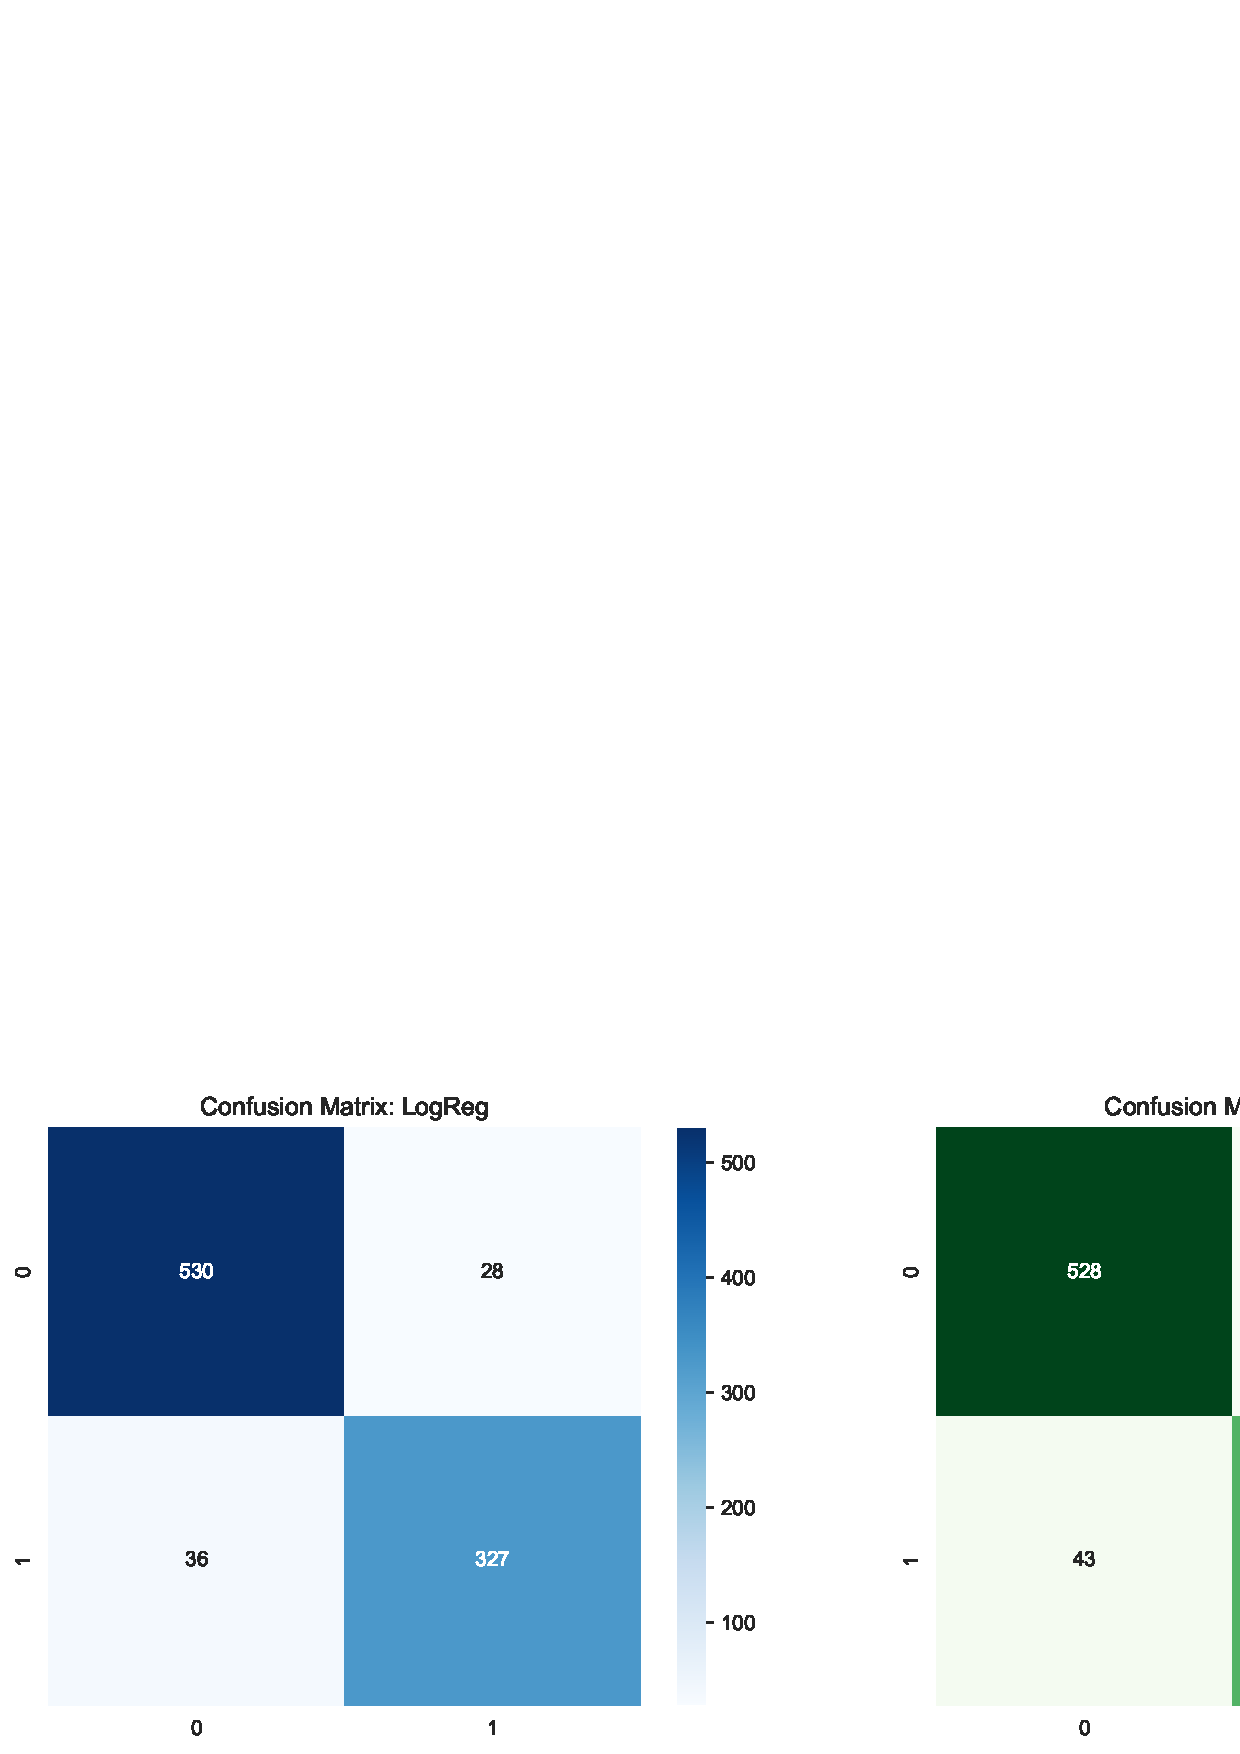
\includegraphics[width=1.0\textwidth]{Images/PNG/confusion_matrices.png}
    \caption{Confusion Matrix Comparison (DT vs RF)}
\end{figure}

\begin{figure}[H]
    \centering
    \includegraphics[width=0.8\textwidth]{Images/PNG/roc_comparison.png}
    \caption{ROC Curve Comparison}
\end{figure}

%--------------------------------------------------

\section*{Observations}
\begin{itemize}
    \item \textbf{How does tree depth affect overfitting in Decision Trees?} \\
    Shallow trees can underfit the data. As the depth increases, the tree begins to memorize the training data (including noise), leading to overfitting and high variance. Tuning `max\_depth` restricts this growth, forcing the model to capture only the most significant patterns.
    
    \item \textbf{Which hyperparameter had the greatest impact on performance?} \\
    For the Decision Tree, `max\_depth` and `min\_samples\_leaf` heavily influenced pruning and prevented overfitting. For the Random Forest, `n\_estimators` (number of trees) had the most stabilizing effect on test accuracy.
    
    \item \textbf{How does Random Forest improve generalization?} \\
    By generating multiple decision trees trained on random subsets of the data (bootstrapping) and considering random subsets of features at each split, it ensures that trees are largely uncorrelated. Averaging their predictions dramatically reduces variance.
    
    \item \textbf{Did ensemble learning always improve performance? Why or why not?} \\
    Yes, for this complex diagnostic dataset. Test accuracy improved from 94.74\% (DT) to 96.49\% (RF). However, if base learners are highly correlated or the dataset is extremely simplistic, the computational overhead of an ensemble might not yield a massive gain over a single fine-tuned tree.
\end{itemize}

%--------------------------------------------------

\section*{Conclusion}
Decision Tree and Random Forest models were implemented and evaluated using 5-fold cross-validation. Hyperparameters were effectively selected using \texttt{GridSearchCV} based on average cross-validation performance, ensuring robust generalization. The results definitively demonstrate that the Random Forest reduces model variance and improves stability compared to a single Decision Tree, achieving higher accuracy (96.49\%) and a more robust AUC score on the Wisconsin Diagnostic Breast Cancer Dataset.

%--------------------------------------------------

\section*{References}
\begin{itemize}
    \item \href{https://scikit-learn.org/stable/modules/tree.html}{Scikit-learn: Decision Trees}
    \item \href{https://scikit-learn.org/stable/modules/ensemble.html}{Scikit-learn: Random Forest}
    \item \href{https://archive.ics.uci.edu/dataset/17/breast+cancer+wisconsin+diagnostic}{UCI Dataset: Breast Cancer Wisconsin (Diagnostic)}
\end{itemize}

\end{document}